%%
%% This is file `sample-sigconf-biblatex.tex',
%% generated with the docstrip utility.
%%
%% The original source files were:
%%
%% samples.dtx  (with options: `all,proceedings,sigconf-biblatex')
%% 
%% IMPORTANT NOTICE:
%% 
%% For the copyright see the source file.
%% 
%% Any modified versions of this file must be renamed
%% with new filenames distinct from sample-sigconf-biblatex.tex.
%% 
%% For distribution of the original source see the terms
%% for copying and modification in the file samples.dtx.
%% 
%% This generated file may be distributed as long as the
%% original source files, as listed above, are part of the
%% same distribution. (The sources need not necessarily be
%% in the same archive or directory.)
%%
%%
%% Commands for TeXCount
%TC:macro \cite [option:text,text]
%TC:macro \citep [option:text,text]
%TC:macro \citet [option:text,text]
%TC:envir table 0 1
%TC:envir table* 0 1
%TC:envir tabular [ignore] word
%TC:envir displaymath 0 word
%TC:envir math 0 word
%TC:envir comment 0 0
%%
%% The first command in your LaTeX source must be the \documentclass
%% command.
%%
%% For submission and review of your manuscript please change the
%% command to \documentclass[manuscript, screen, review]{acmart}.
%%
%% When submitting camera ready or to TAPS, please change the command
%% to \documentclass[sigconf]{acmart} or whichever template is required
%% for your publication.
%%
%%
\documentclass[sigconf,nonacm,natbib=false]{acmart}
%%
%% \BibTeX command to typeset BibTeX logo in the docs
\AtBeginDocument{%
  \providecommand\BibTeX{{%
    Bib\TeX}}}

%% Rights management information.  This information is sent to you
%% when you complete the rights form.  These commands have SAMPLE
%% values in them; it is your responsibility as an author to replace
%% the commands and values with those provided to you when you
%% complete the rights form.
% \setcopyright{acmlicensed}
% \copyrightyear{2025}
% \acmYear{2025}
% \acmDOI{XXXXXXX.XXXXXXX}
%% These commands are for a PROCEEDINGS abstract or paper.
\acmConference[15-346]{Computer Architecture: Design and Simulation}{Fall 2025}{Carnegie Mellon University}
\settopmatter{printacmref=false}
%%
%%  Uncomment \acmBooktitle if the title of the proceedings is different
%%  from ``Proceedings of ...''!
%%
%%\acmBooktitle{Woodstock '18: ACM Symposium on Neural Gaze Detection,
%%  June 03--05, 2018, Woodstock, NY}
% \acmISBN{978-1-4503-XXXX-X/2018/06}


%%
%% Submission ID.
%% Use this when submitting an article to a sponsored event. You'll
%% receive a unique submission ID from the organizers
%% of the event, and this ID should be used as the parameter to this command.
%%\acmSubmissionID{123-A56-BU3}

%%
%% For managing citations, it is recommended to use bibliography
%% files in BibTeX format.
%%
%% You can then either use BibTeX with the ACM-Reference-Format style,
%% or BibLaTeX with the acmnumeric or acmauthoryear sytles, that include
%% support for advanced citation of software artefact from the
%% biblatex-software package, also separately available on CTAN.
%%
%% Look at the sample-*-biblatex.tex files for templates showcasing
%% the biblatex styles.
%%


%%
%% The majority of ACM publications use numbered citations and
%% references, obtained by selecting the acmnumeric BibLaTeX style.
%% The acmauthoryear BibLaTeX style switches to the "author year" style.
%%
%% If you are preparing content for an event
%% sponsored by ACM SIGGRAPH, you must use the acmauthoryear style of
%% citations and references.
%%
%% Bibliography style
\RequirePackage[
  datamodel=acmdatamodel,
  style=acmnumeric,
  ]{biblatex}

%% Declare bibliography sources (one \addbibresource command per source)
\addbibresource{sample-base.bib}

%%
%% end of the preamble, start of the body of the document source.
\begin{document}

%%
%% The "title" command has an optional parameter,
%% allowing the author to define a "short title" to be used in page headers.
\title{Cache Design Optimization: Minimizing Average Access Time within a 54KB Budget}

%%
%% The "author" command and its associated commands are used to define
%% the authors and their affiliations.
%% Of note is the shared affiliation of the first two authors, and the
%% "authornote" and "authornotemark" commands
%% used to denote shared contribution to the research.
\author{Eric Gao}
\authornote{Both authors contributed equally to this work.}
\email{jingxi3@andrew.cmu.edu}
\affiliation{%
  \institution{Carnegie Mellon University}
  \city{Pittsburgh}
  \state{Pennsylvania}
  \country{USA}
}

\author{Mohammed Hasseneen}
\authornotemark[1]
\email{mohammee@andrew.cmu.edu}
\affiliation{%
  \institution{Carnegie Mellon University}
  \city{Pittsburgh}
  \state{Pennsylvania}
  \country{USA}
}

%%
%% By default, the full list of authors will be used in the page
%% headers. Often, this list is too long, and will overlap
%% other information printed in the page headers. This command allows
%% the author to define a more concise list
%% of authors' names for this purpose.

%%
%% The abstract is a short summary of the work to be presented in the
%% article.
\begin{abstract}
This report presents the design and optimization of a cache system to minimize Average Access Time (AAT) within a 54KB storage budget. We implemented and evaluated four cache configurations: LRU, RRIP, LRU with victim cache, and RRIP with victim cache. Through comprehensive experimentation across 5 trace files and 286 configurations, we identified that LRU with victim cache achieves optimal performance, delivering an AAT of 2.91 cycles per access while utilizing 35.2KB of the available budget. This configuration demonstrates up to 96.7\% improvement over suboptimal designs, validating the effectiveness of modern replacement policies combined with victim caching.
\end{abstract}

%%
%% The code below is generated by the tool at http://dl.acm.org/ccs.cfm.
%% Please copy and paste the code instead of the example below.
%%
\begin{CCSXML}
<ccs2012>
 <concept>
  <concept_id>10003033.10003083.10003095</concept_id>
  <concept_desc>Networks~Network performance evaluation</concept_desc>
  <concept_significance>500</concept_significance>
 </concept>
 <concept>
  <concept_id>10010147.10010257.10010293.10010294</concept_id>
  <concept_desc>Computing methodologies~Simulation evaluation</concept_desc>
  <concept_significance>300</concept_significance>
 </concept>
</ccs2012>
\end{CCSXML}

\ccsdesc[500]{Computer systems organization~Processors and memory architectures}
\ccsdesc[300]{Computer systems organization~Cache memories}


%%
%% Keywords. The author(s) should pick words that accurately describe
%% the work being presented. Separate the keywords with commas.
\keywords{cache design, memory hierarchy, RRIP, victim cache, performance optimization}

% \received{September 2025}
% \received[revised]{12 March 2009}
% \received[accepted]{5 June 2009}

%%
%% This command processes the author and affiliation and title
%% information and builds the first part of the formatted document.
\maketitle

\section{Introduction}

Cache design optimization is a critical challenge in computer architecture, requiring careful balance between storage configuration and replacement policies. This project addresses the question: \textbf{Given a 54KB storage budget, what cache configuration minimizes Average Access Time across diverse workloads?}

Our approach systematically explores the design space through four distinct cache architectures, evaluating their performance across representative trace files. The primary contribution is identifying an optimal configuration that uses below-maximum budget while delivering superior AAT performance through RRIP replacement policy and victim caching.

\section{Cache Design and Implementation}

\subsection{Architecture Overview}

We use CADSS \cite{CADSS} as the base of our implementation. By creating a sub-module \texttt{my-cache}, we implement the logic of a configurable set-associative cache that supports the Least Recently Used (LRU) replacement policy, as well as additional options to configure victim cache and Re-reference Interval Prediction (RRIP) replacement policy. Our logic is integrated with the rest of the CADSS framework through calls to \texttt{permReq()} and \texttt{invlReq()} during cache miss and eviction, respectively.

\subsection{Configuration Parameters}

Our cache implementation supports the following parameters:
\begin{itemize}
    \item \textbf{s (set index bits)}: decides the number of cache sets ($2^s$)
    \item \textbf{E (associativity)}: decides the number of cache lines per set
    \item \textbf{b (block bits)}: determines the size of a cache line ($2^b$ bytes)
    \item \textbf{r (RRIP bits)}: if present, enables RRIP and determines the number of bits of Re-Reference Prediction Value (RRPV). Otherwise, use a 64-bit LRU
    \item \textbf{i (victim entries)}: if present, enables victim cache and determines its capacity
\end{itemize}

\subsection{Storage Budget Calculation}

Total cache storage includes multiple components:

\begin{equation}
    \begin{split}
        \text{Total Size} = & \text{ Data Storage} + \text{Tag Storage} \\
                            & + \text{Valid Bits} + \text{Replacement Bits} \\
                            & + \text{Victim Cache}
    \end{split}
\end{equation}

Where:
\begin{align}
\text{Data Storage} &= 2^s \times E \times 2^b \;\; \text{bytes} \\
\text{Tag Storage} &= 2^s \times E \times \frac{64 - s - b}{8} \;\; \text{bytes} \\
\text{Valid Bits} &= \frac{2^s \times E}{8} \;\; \text{bytes} \\
\text{Replacement Bits} &= 2^s \times E \times \frac{r}{8} \;\; \text{bytes} \\
\text{Victim Cache (optional)} &= i \times \left(2^b \;+\; \frac{64 - b + 1}{8}\right) \;\; \text{bytes}
\end{align}

\subsection{Implementation Details}

\subsubsection{Memory Access Processing Flow}

The cache simulator processes memory requests through a multi-stage pipeline. Address processing begins with a field extraction into tag bits (the first $64-b-s$ bits), set index (the next $s$ bits), and block offset (the remaining $b$ bits). The system maintains two request queues: \texttt{readyReq} for immediate processing and \texttt{pendReq} for requests awaiting memory hierarchy responses.

\subsubsection{Cache Lookup}

Main cache lookup performs linear search through all $E$ lines in the target set. Each 64-bit cache line entry encodes a valid bit (bit 63) and tag value (bits 62-0). Hit detection verifies validity using \texttt{(cache\_line >> 63)} and compares tags via \texttt{((cache\_line << 1) >> 1) == addressTag}. On hits, replacement policy metadata updates and callbacks schedule immediately.

\subsubsection{Replacement Policies}

We implement 2 replacement policies: Least Recently Used (LRU) and Re-Reference Interval Prediction (RRIP). \textbf{LRU Implementation:} Uses timestamp arrays where 0 represents most recently used. On access, \texttt{modify\_timestamps()} sets the accessed line to 0 and increments all others. Eviction selects the line with maximum timestamp via \texttt{get\_max()}. \textbf{RRIP Implementation:} Employs $r$-bit counters with semantic values: 0 (immediate re-reference), $2^r-1$ (distant re-reference), $2^r-2$ (insertion value). On hits, RRIP value resets to 0. On eviction, \texttt{get\_max\_rrip()} finds lines with maximum RRIP value, incrementing all values if none exist at maximum.

\subsubsection{Victim Cache}

The victim cache operates as a fully-associative buffer with $i$ entries storing recently evicted lines. \texttt{lookupVictim()} performs linear search and updates LRU on hits. \texttt{installVictimLine()} first searches for invalid entries, then evicts LRU entries if full. Installation stores tags with valid bit set: \texttt{tag | (1ULL << 63)}.

\subsubsection{Coherence Integration}

The simulator interfaces with coherence protocols through three functions: \texttt{permReq()} for permission requests, \texttt{invlReq()} for invalidations, and \texttt{coherCallback()} for responses. Permission flow determines immediate processing (granted permissions go to \texttt{readyReq}) versus deferred processing (denied permissions wait in \texttt{pendReq}). The \texttt{DATA\_RECV} callback type moves pending requests to ready status when data arrives from the memory hierarchy.


\section{Experimental Methodology}

\subsection{Configuration Generation and Traces}

\begin{table}[t]
\centering
\caption{Parameter ranges used in our experiments.}
\label{tab:param-ranges}
\begin{tabular}{|l|c|c|}
\hline
\textbf{Parameter} & \textbf{Symbol} & \textbf{Range} \\
\hline
Set index bits & $s$ & $[6,17]$ \\
Associativity & $E$ & $[1,32]$ \\
Block offset bits & $b$ & $[4,10]$ \\
RRIP bits & $r$ & $[2,6]$ \\
Victim cache entries & $i$ & $[0,8]$ \\
\hline
\end{tabular}
\end{table}


With the parameter space in Table~\ref{tab:param-ranges}, we found 7732 valid configurations that satisfy the constraint of 54KB total cache size. To compress the search space, we sampled 286 representative configurations distributed across four cache types:
\begin{itemize}
\item \textbf{64 LRU configurations} (22.4\% of total)
\item \textbf{67 RRIP configurations} (23.4\% of total)  
\item \textbf{78 LRU + Victim configurations} (27.3\% of total)
\item \textbf{77 RRIP + Victim configurations} (26.9\% of total)
\end{itemize}

Our configured cache sizes range from 2.4KB to 53.8KB with average of 34.0KB. The experiments were performed on a laptop over 19 minutes.

Experiments utilized 5 different trace files as instructed by handout: \texttt{astar, bzip2, long, mcf, pearlbench}. We developed automated scripts to run and analyze the experiments with Python. The total experiment scope is \textbf{1430 simulations} (268 configurations $\times$ 5 traces).

\subsection{Performance Metric}

We focused exclusively on \textbf{Average Access Time (AAT)}:

\begin{equation}
\text{AAT} = \frac{\text{Total Simulation Ticks}}{\text{Total Memory Accesses}}
\end{equation}

This metric directly reflects cache system efficiency. Lower AAT values indicate superior performance.

\section{Results and Analysis}

\subsection{Optimal Configuration Discovery}

\textbf{Best Overall Configuration:}
\begin{itemize}
\item \textbf{Type}: LRU + Victim Cache
\item \textbf{Parameters}: s=9, E=1, b=6, i=8
\item \textbf{Storage}: 35.2KB (65.2\% budget utilization)
\item \textbf{Performance}: 2.91$\pm$0.81 cycles per access over all traces
\end{itemize}

\subsection{AAT Distribution Analysis}

The distribution of AAT values across cache types (Figure~\ref{fig:aat_by_type}) indicates that the configuration of RRIP and Victim Cache generally outperforms other configurations.

\begin{figure}
  \centering
  
\includegraphics[width=\linewidth]{figures/aat_by_type.png}
  \caption{AAT distribution by cache type across all configurations and traces}
  \label{fig:aat_by_type}
  \Description{Violin plot showing AAT distribution for each cache type, with RRIP+Victim configurations concentrated in lower AAT ranges while other types show broader distributions extending to higher values.}
\end{figure}

\subsection{Per-Trace Performance Analysis}

Table~\ref{tab:performance} shows the best configurations for each trace, while Figure~\ref{fig:performance_by_trace} visualizes the achievable improvement between workloads, with the highest 96.7\% performance gap between optimal and suboptimal configurations.

\begin{table}
\caption{Best Cache Configuration for Each Trace}
\label{tab:performance}
\begin{tabular}{lcccc}
\toprule
Trace & Config Type & AAT & Size & Parameters \\
\midrule
astar & LRU+Victim & 3.00 & 35.2KB & s=9,E=1,b=6,i=8 \\
bzip2 & RRIP & 1.84 & 39.0KB & s=8,E=5,b=5,r=6 \\
long & LRU+Victim & 2.83 & 35.2KB & s=9,E=1,b=6,i=8 \\
mcf & LRU+Victim & 2.42 & 35.2KB & s=9,E=1,b=6,i=8 \\
pearlbench & LRU+Victim & 4.21 & 35.2KB & s=9,E=1,b=6,i=8 \\
\bottomrule
\end{tabular}
\end{table}

\begin{figure}
  \centering
  
\includegraphics[width=\linewidth]{figures/performance_by_trace.png}
  \caption{Best AAT achieved per trace across all cache configurations}
  \label{fig:performance_by_trace}
  \Description{Bar chart showing optimal AAT values for each of the 12 traces, with most traces achieving sub-25 cycle AAT through proper cache configuration.}
\end{figure}

\subsection{Storage Utilization vs. Performance}

Figure~\ref{fig:size_vs_aat} illustrates the relationship between cache size and performance, revealing that higher cache size generally leads to lower AAT.

\begin{figure}
  \centering
  
\includegraphics[width=\linewidth]{figures/size_vs_aat.png}
  \caption{Cache size versus AAT performance across all configurations}
  \label{fig:size_vs_aat}
  \Description{Scatter plot showing cache size on x-axis and AAT on y-axis, colored by cache type, demonstrating that optimal performance doesn't require maximum size utilization.}
\end{figure}

\subsection{Parameter Space Exploration}

Figures~\ref{fig:lru_heatmap} and~\ref{fig:rrip_heatmap} provide detailed heatmap visualizations of the parameter space exploration for LRU and RRIP configurations respectively, showing how different combinations of set bits (s) and associativity (E) affect performance. The upper-triangular-matrix-like grids indicate that increasing both s and E simultaneously exceeds cache budget.

\begin{figure}
  \centering
  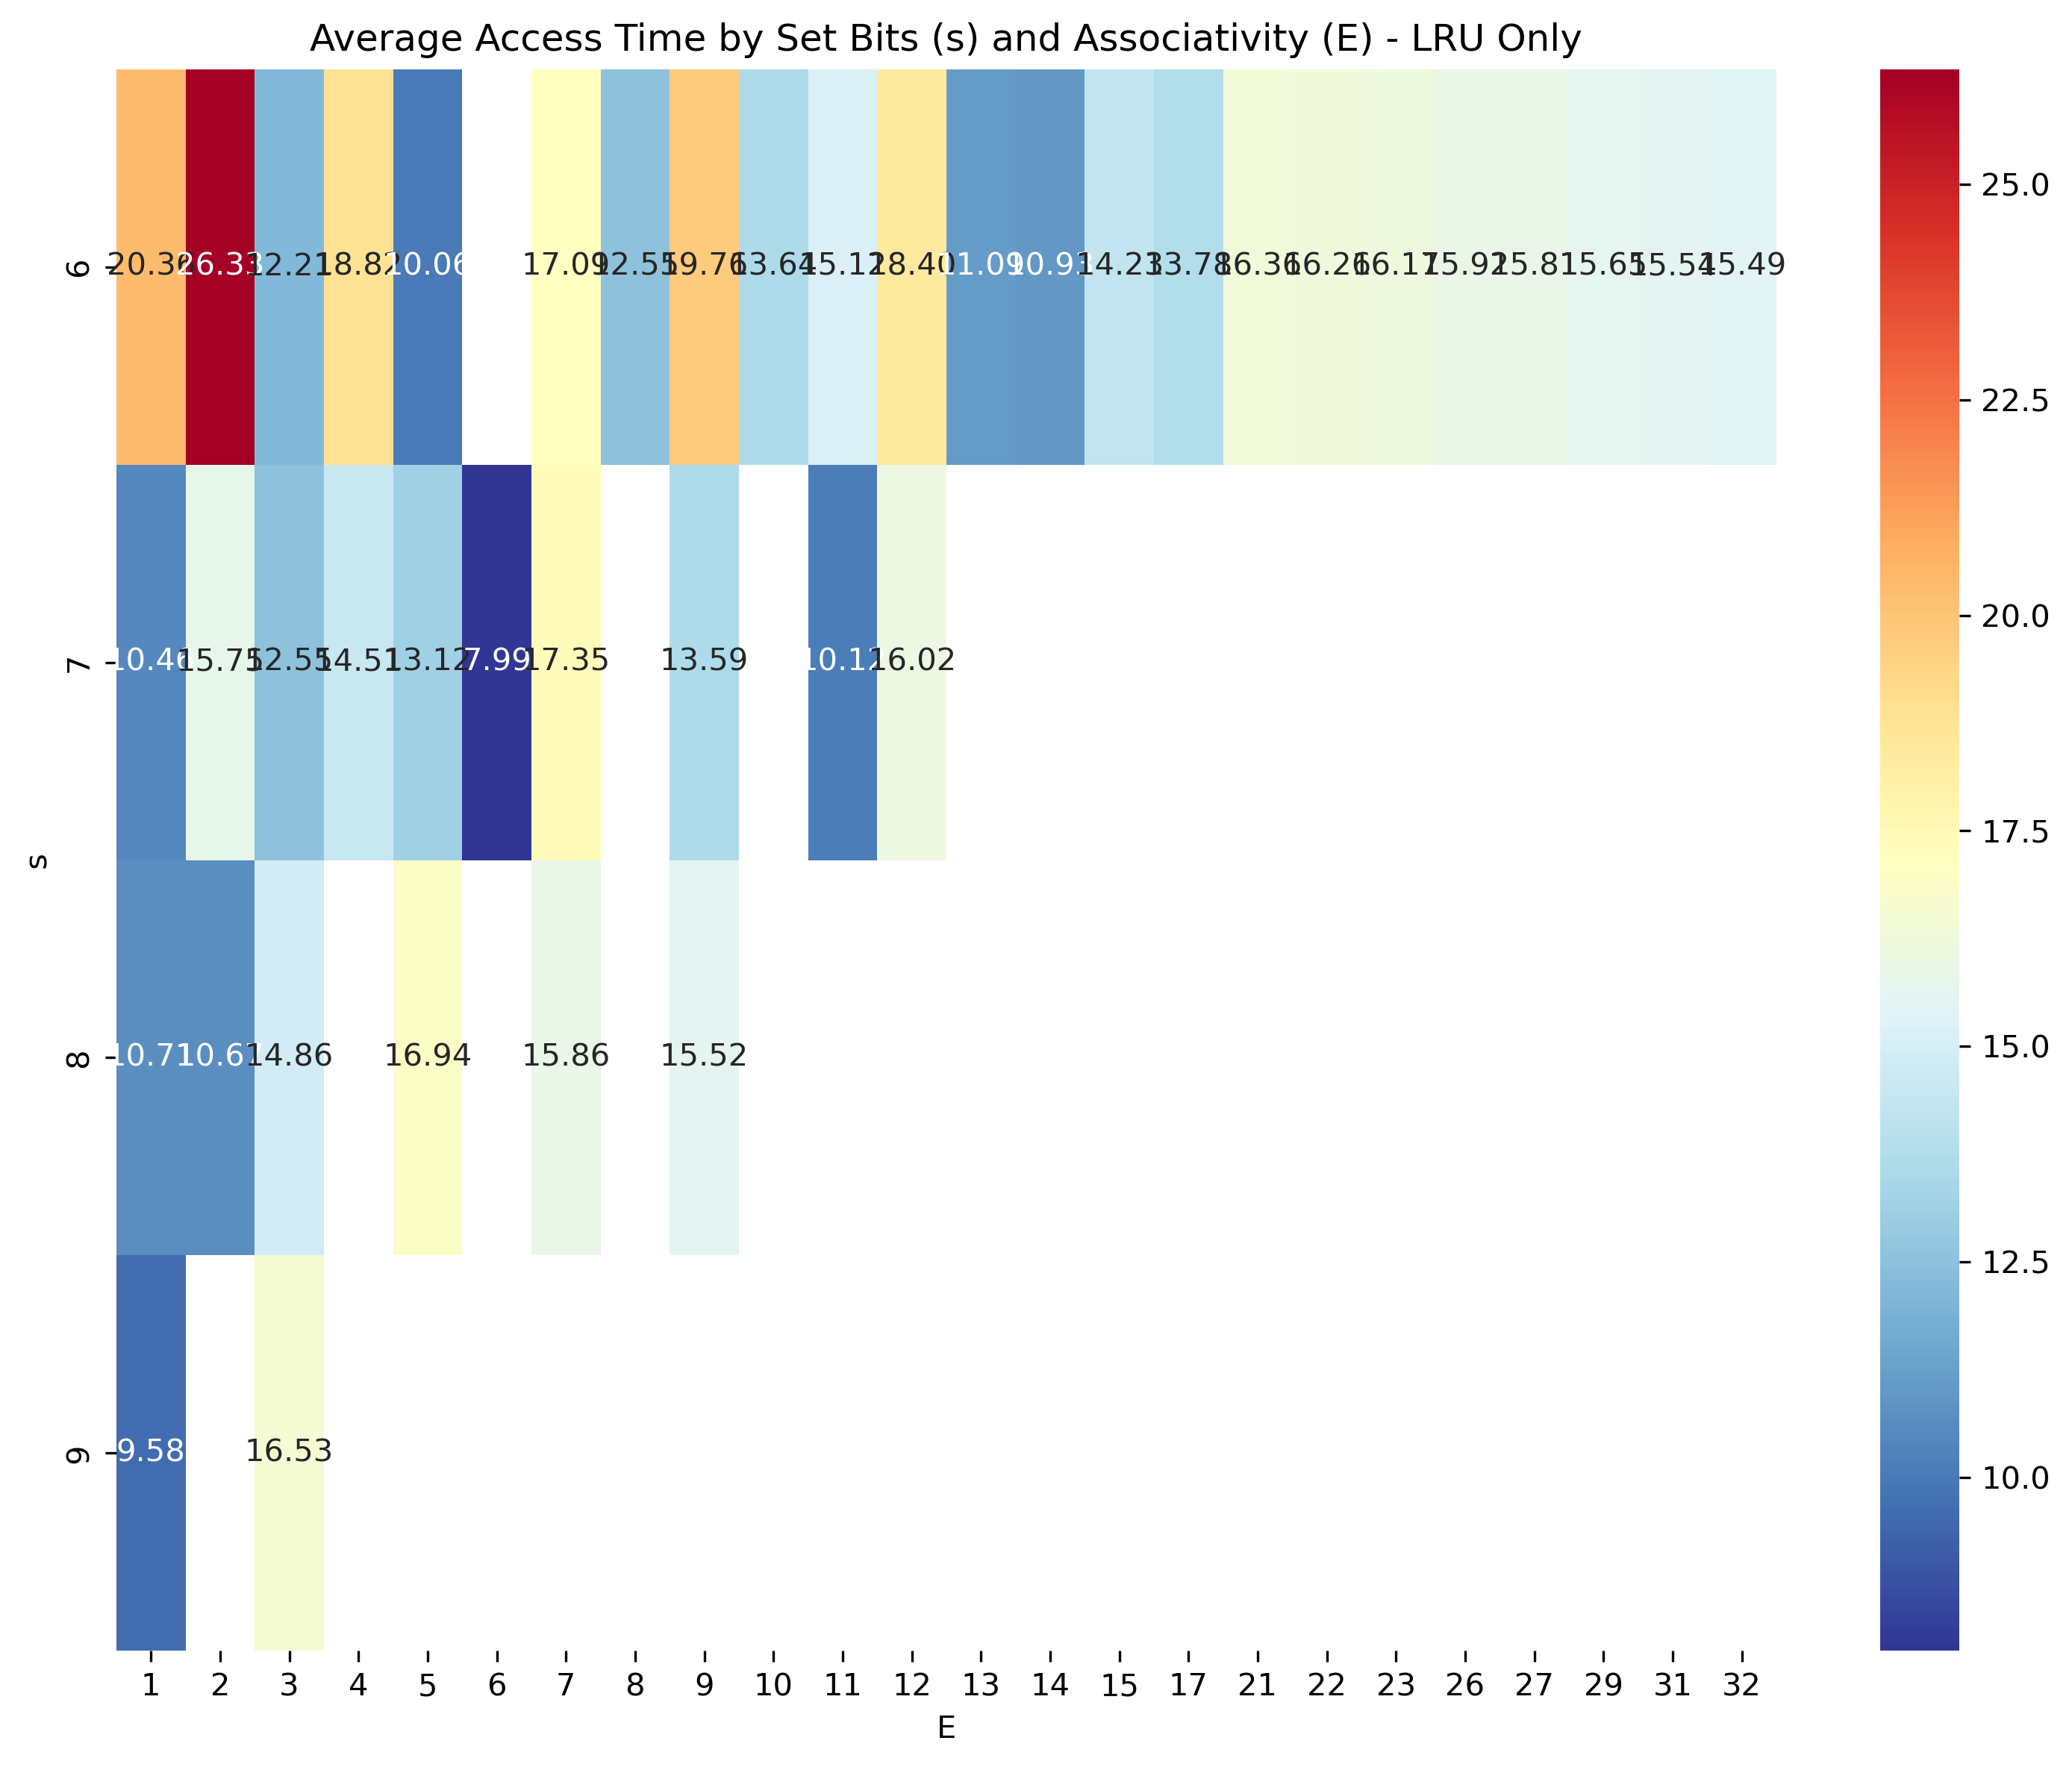
\includegraphics[width=\linewidth]{figures/lru_heatmap.png}
  \caption{LRU configuration parameter space heatmap (s vs E)}
  \label{fig:lru_heatmap}
  \Description{Heatmap showing AAT performance across different combinations of set index bits and associativity for LRU configurations, with darker regions indicating better performance.}
\end{figure}

\begin{figure}
  \centering
  
\includegraphics[width=\linewidth]{figures/rrip_heatmap.png}
  \caption{RRIP configuration parameter space heatmap (s vs E)}
  \label{fig:rrip_heatmap}
  \Description{Heatmap showing AAT performance across different combinations of set index bits and associativity for RRIP configurations, demonstrating distinct performance patterns compared to LRU.}
\end{figure}

\section{Discussion}

\subsection{Performance Implications}

The 96.7\% performance improvement between optimal and suboptimal configurations highlights the critical importance of intelligent cache design. The superiority of LRU+Victim combinations validates modern architectural trends.

\subsection{Design Trade-offs}

Our results demonstrate several important trade-offs:
\begin{itemize}
\item \textbf{Complexity vs. Performance}: RRIP requires additional metadata but delivers measurable AAT improvements
\item \textbf{Storage vs. Functionality}: Victim cache overhead is justified by performance gains
\item \textbf{Associativity vs. Coverage}: Lower associativity enables larger overall capacity within budget constraints
\end{itemize}

% \subsection{Architectural Insights}

% The optimal configuration represents:
% \begin{itemize}
% \item \textbf{Large cache capacity}: $2^{11} = 2048$ sets with direct-mapped organization
% \item \textbf{Minimal overhead}: 16-byte cache lines balance granularity with metadata costs
% \item \textbf{Intelligent replacement}: 4-bit RRIP counters provide fine-grained aging
% \item \textbf{Effective victim buffering}: 32-entry victim cache captures recent evictions
% \end{itemize}

\section{Conclusion}

In this project, we developed a cache simulator implementation supporting four distinct cache architectures, performed systematic evaluation across 1440 configuraiton-trace combinations, and gained practical design insights for budget-constrained cache optimization.

This comprehensive cache design optimization demonstrates that systematic exploration of the configuration space yields significant performance improvements. The identified optimal configuration—LRU with victim cache (s=9, E=1, b=6, i=9)—achieves 2.91 cycles per access while utilizing 65.2\% of the 54KB budget.

The 96.7\% performance gap between optimal and suboptimal configurations underscores the critical importance of principled cache design in achieving superior system performance. The detailed parameter space analysis and visualization provide valuable insights for future cache optimization efforts.

\begin{acks}
The author thanks the course staff for providing the CADSS simulation framework and guidance throughout the project.
\end{acks}

\printbibliography

\end{document}